%Waves Program Master Degree Template
%Author: Viktoriia Boichenko
%vik.boichenko@gmail.com

% !TEX encoding = UTF-8 Unicode
% !TEX TS-program = xelatex

\documentclass[11pt]{article}

% Language setting
\usepackage[english]{babel}
\usepackage{fontspec}
% \setmainfont{Arial}
% Set page size and margins
\usepackage[letterpaper,top=2.54cm,bottom=2.54cm,left=3.27cm,right=3.27cm,marginparwidth=1.75cm]{geometry}
% Set spacing between lines and sections
\usepackage{titlesec}
\titlespacing*{\section}{0pt}{32pt}{20pt}
\titlespacing*{\subsection}{0pt}{16pt}{20pt}
\usepackage{setspace}
\onehalfspacing
%Adds space after paragraph
\usepackage{parskip}
\setlength{\parindent}{0pt}

% Useful packages
\usepackage{amsmath}
\usepackage{graphicx}
\usepackage[colorlinks=true, allcolors=blue]{hyperref}
\usepackage{units}
\usepackage{multirow}
\usepackage{caption}
\usepackage{csquotes}
\usepackage{float} %locate figures with [H]

%Import the bibliography file
\usepackage[backend=biber,style=ieee]{biblatex}
\addbibresource{bibliography.bib} 


\begin{document}

%setting the cover page
\thispagestyle{empty}
% \begin{minipage}{0.96\linewidth}
% \includegraphics[width=1\linewidth]{figures/gandia-upv.png}
% \end{minipage}

\begin{center}
{\large\text{Erasmus Mundus WAVES}}   \\
{\large\text{GEOMAR, DeepSeaMonitoring}}   

{\Large\textbf{Report \\ }}   

 {\Large\text{Viktoriia Boichenko}} 

{\large\text{2023/2024}}   
\end{center}

\tableofcontents

\section{Introduction}


The goal of this report is an overview of the literature covered in the scope of the research on the acoustic response of the bubble along with the results of different implementations.

This report is structured with a theoretical part and practical sections. Theoretical includes the following subsections:
\begin{itemize}
	\item sound propagation basic concepts
	\item general SONAR principles and systems. The basics of acoustic wave propagation are explained and techniques utilized in SONAR systems
	\item beamforming and matched filtering
	\item cross-section scattering, backscattering, single and multiple scattering, 
	\item natural frequency provided by bubble, 
	\item single bubble model present in the literature (Thuraisigham).  
	% \item Minaert frequency, Rayleigh-Plesset equation of air bubble. 
\end{itemize}
The practical part includes the following subsections:
\begin{itemize}
	\item Calculation: After that the results of the implementation of a single bubble model are shown. 
	\item Results and the interpretation of them and further developments are described as well. 
\end{itemize}
In the end, the conclusion provides a summary of the whole report.
\subsection{Literature review}

\textbf{About single bubble modelling} 
(Manasseh et al. 2004 \cite{manasseh_anisotropy_2004}) Bubbles produce an acoustic signal owing to compression of the gas in the bubble. The ‘spring’ of the compressible gas and the mass of liquid around the bubble create a natural oscillator, sending a pressure oscillation through the liquid and interacting with the neighbouring bubbles

(Zhang et al. 2022 \cite{zhang_efficient_2022} ) This paper provides a volume-scattering strength optimization model. This model allows to estimate the bubble size distribution. It provides a thorough explanation with the help of the case study experiment with a multibeam sonar to identify a bubble leakage in the sea.

It identifies three parameters: two in probability density function of gas leakage bubble sizes and the total number of bubbles inside the sample volume N0. Direct method was used for obtaining parameters.

(Li et al. 2020 \cite{li_broadband_2020}) Mentions theory regarding the bubble size distribution and provides the data for the backscattering cross-section of a single bubble. The model of the bubble plume’s acoustic backscattering consists of the model of the single bubble, distribution of size of the bubbles and computation of the volume scattering strength.

\section{Theoretical part}
\subsection{Sound propagation}
The wave’s acoustic energy is assumed to be uniformly distributed over the area $4\pi r^{2}$ of a sphere with the radius $r$. Therefore, the \textbf{acoustic intensity} at the distance r from the source is given by Equation \ref{eqn:ac_intensity}:
\begin{equation} 
\label{eqn:ac_intensity}
I(r) = \frac{P}{4\pi r^{2}}
\end{equation}
with the radiated power P of the source, measured in Watt.

As the acoustic wave propagates forward, mainly two types of propagation losses occur, with respect to the wave’s intensity:
\begin{itemize}
\item \textbf{the geometric spreading loss} is related to the quadratic increase in the sphere’s surface with the rise of the propagation distance. 

The transmitted acoustic energy is conserved but distributed over an increased surface area. This results in a decrease in the acoustic intensity.
\item \textbf{the absorption loss} is caused by the dissipation of acoustic energy.
As seawater is a dissipative propagation medium \cite{lurton2002introduction}, parts of the acoustic wave’s energy are absorbed due to water viscosity (for sound frequencies of order 1MHz) and chemical relaxation effects (for frequencies up to 300kHz)  \cite{ainslie_principles_2010}. This causes an exponential decrease in the acoustic pressure of the wave, proportional to the increasing propagation distance
\end{itemize}

\textbf{The transmission loss (TL)} is the loss in SNR due to the propagation losses. Assuming the simplification of non-absorbing water, the formula of the transmission loss for the modelling of the spherical spreading loss at the propagation distance $r$  is given by:
\begin{equation}
TL_{spherical} = 20\log_{10}r
\label{eq:transmission_loss_sph}
\end{equation}

The cylindrical spreading loss takes into account that the propagating acoustic waves are bounded by two parallel planes, the bottom and surface of the sea:
\begin{equation}
TL_{cylindrical} = 10\log_{10}r
\label{eq:transmission_loss_cyl}
\end{equation}

\textbf{The target strength (TS)} is a measure for the reflection strength of a target object. It is given by the ratio of the incident acoustic intensity $I_{i}(r)$, compared to the reflected acoustic intensity $I_{r}(r)$
\begin{equation}
TS = 10\log_{10}\frac{I_r}{I_i}
\label{eq:target_strength_gen}
\end{equation}

\subsection{SONAR}

	SONAR is an echo-ranging device emitting and receiving sound wave signals to investigate the water surroundings. The acronym stands for sound navigation ranging. There are active and passive types of sonar, where only the first one can transmit the signal, while both can receive it.
	
	The operation of an active SONAR is based on the use of transmitting projectors and receiving hydrophones. The projector converts a transmit signal to acoustic pressure waves, which emit from the projector's location and propagate through a physical medium like water, gas or solids \cite{hodges_underwater_2011}. The transmission energy of the SONAR can be focused in a wanted direction by using beamforming. The transmitted waves get reflected by backscattering objects and are recorded by receiving hydrophones. To detect the transmitted signals in the received signals, the matched filter can be applied. Applying the principle of echolocation \cite{ainslie_principles_2010}, the distance to and direction of backscattering objects can be determined by analyzing the time delay and phase relations between the transmitted and received signals.
	
	The fields of usage: communication, detection or characterization of objects.
	
	\begin{figure} [H][htbp] %  figure placement: here, top, bottom, or page
	   \centering
	   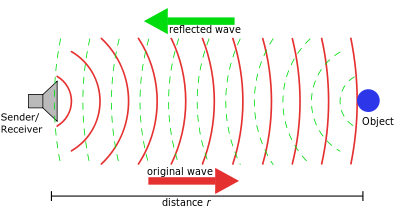
\includegraphics[width=0.6\linewidth]{figures/sonar_scheme.png} 
	   \caption{A scheme of the sonar principle of work}
	   \label{fig:sonar_scheme}
	\end{figure}
	
\subsection{Beamforming}
	The transmission energy of the SONAR can be focused in a wanted direction by using beamforming. The general idea of beamforming is to process receive and/or transmit signals, using an array with multiple receivers or transmitters, to achieve an SNR gain by constructive superposition. The processing depends on the geometric alignment of the array elements and the steering of the formed beam into the target direction. Signals coming from the wanted direction are added in phase, causing the amplification of the wanted signal components, while signals from unwanted directions are attenuated by destructive interference.

The spatial filter is called a beamformer as it allows to amplify selectively the arriving signal to each receiver from a narrow range of angles \cite{hodges_underwater_2011}.
	
	The delay-and-sum beamformer where each of the $N_{R_x}$ output signal $y_m(n)$ recorded by the m-th hydrophone is delayed by a number of samples, which can be calculated with the following formula:
\begin{equation}
\tau_m=\frac{d_m sin(\varphi_s)}{c}f_s
\label{eqn:delay-and-sum-beam-delay}
\end{equation}

\begin{figure} [H][htbp] %  figure placement: here, top, bottom, or page
   \centering
   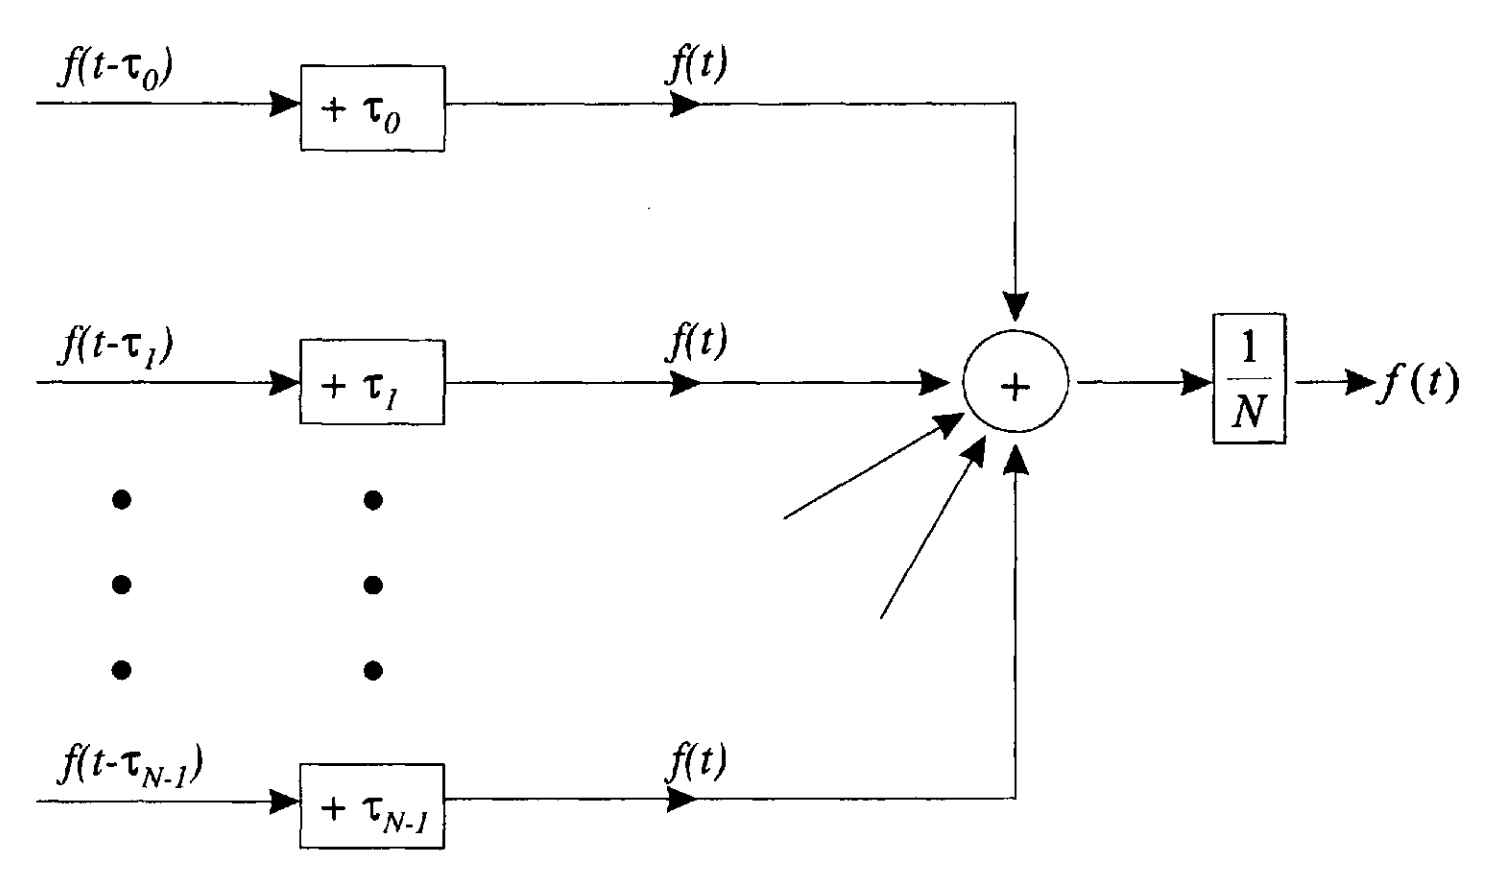
\includegraphics[width=0.8\textwidth]{figures/delay-and-sum.png} 
   \caption{Delay-and-sum beamformer \cite{trees_optimum_2002}}
   \label{fig:delay-and-sum}
\end{figure}

\subsection{Matched filtering}

The matched filter is used for detecting the presence of the known transmit signal $x(n)$ in a noisy receive signal $y(n)$. It is optimal for detecting a waveform in the presence of white noise. For the signal $x(n)$ of length $n \in 0, ..., N_x − 1$, the impulse response of the matched filter
\[h(n) = x(N_x − 1 − n)\] is given by the time-reversal of the signal $x(n)$. The output of the matched filter is then given by the convolution sum:
\begin{equation}
y_{mf}(n) = y(n)*h(n) = \sum_{k=0}^{N_y-1}y(k)h(n-k)
\end{equation}
between the received signal $y(n)$ of length $n \in 0, \ldots , N_y − 1$ and the impulse response of the matched filter. The output of the matched filter is a measure for the resemblance of the target signal $x(n)$ in the received signal $y(n)$ at time $n$, being maximal if both signals align.

This measure of similarity between two stationary random processes $x(n)$ and $y(n)$ at lag $l$ is defined by the cross-correlation:
\[r_{xy}(l) = E\{x(n + l)y(n)\} \]
Two random process signals are orthogonal if their cross-correlation $r_{xy}(l)$ is zero at all lags.
As this expectation can be difficult to evaluate in practice, it can be estimated by the cross-correlation for deterministic signals.

\subsection{Scattering}

	Scattering from a small object: 
	
	Scattering cross-section -  how much of the incoming wave gets scattered in the direction of the emitter, the ratio of the scattered power to the emitted intensity from a certain grazing angle of an incident plane wave.

 “The scattering cross-section (a,) of a single bubble is the ratio of the time average rate of energy loss from scattering to the incident intensity.” ([Thuraisingham, 1997, p. 2]\cite{thuraisingham_new_1997}
	\[ \sigma_{\theta_{in}} = \frac{W}{I(\theta_{in}}\] where $\sigma$ is the scattered power per unit incident intensity and has dimensions of area.
	
	\[ \sigma_{\Omega}(\theta_{in}; \theta_{out}, \phi ) = \frac{W_{\Omega}(\theta_{out}, \phi )}{I(\theta_{in}}\]  
	


	backscattering: The backscattering cross-section is defined as the differential cross-section evaluated in the backscattering direction, multiplied by $4\pi$
\begin{equation}\label{eq:backscattering}
\sigma^{back}(\theta) =4\pi \sigma_{\Omega}(\theta; \theta, \phi ) 
\end{equation}
	
%		single and multiple scattering, 
	

\subsection{Single bubble model}

	Bubbles produce an acoustic signal owing to compression of the gas in the bubble. The ‘spring’ of the compressible gas and the mass of liquid around the bubble create a natural oscillator, sending a pressure oscillation through the liquid and interacting with the neighbouring bubbles (Manasseh et al. 2004)\cite{manasseh_anisotropy_2004}. This is so called coupled-oscillator theory under the self-consistent approach by describing the collective scattering due to individual bubble interaction with the others

    In the mass-spring model the bubble plays a role of the monopole scatterer which provides accurate results in low-frequency field and derive expressions of resonance characteristics (Feuillade 1995 \cite{feuillade_scattering_1995})

    The equation of motion of the single bubble is given below: 
    \begin{equation}
        m\nu''(t)+b\nu#(t)+\kappa\nu(t)=-P_{inc}e^{-i\omega t}
        \label{eqn:motion-bubble}
    \end{equation}
    which is a an ordinary differential equation representing a mass-spring system for $\nu$ the unknown bubble volume differential \cite{leighton_acoustic_2012}, which is time dependant. \\
    $m=\rho/(4\pi a)$ represents the equivalent mass, \\
    $\rho $ is a liquid density, \\
    $\kappa = 4.2 P_A/(4\pi a^3)$ the bubble stiffness,\\
    $P_A$ the ambient pressure,\\
    $b=\kappa a/c$ the (radiation) damping,\\
    $c$ is a speed of sound in the fluid.

    We consider harmonic wave field solutions:
    \begin{equation}
        \nu(t)=\vec{\nu}e^{-i\omega t}
    \end{equation}

    which leads to the solution of the mass-spring equation \ref{eqn:motion-bubble}:
    \begin{equation}
        \vec{\nu}=\frac{-\frac{P_{inc}}{m\omega^2}}{\frac{\omega_0^2}{\omega}-1-i\delta}
    \end{equation}
	% Consists of calculating the volume of the backscattering strength by the one of models present in the literature (Thuraisingham 1997 \cite{thuraisingham_new_1997}). 
	
	A formula of the backscattering cross-section of an individual bubble, which is valid for a wide range of $ka$. This formula is derived by correcting a final factor reported by Thuraisingham. (Zhang et al. 2022, p. 2-3 \cite{zhang_efficient_2022} )

\begin{equation}\label{eq:volume_backscattering_strength }
	\sigma_{bs} =\frac{a^{2} }{ (\omega_{0}^{2}/\omega^{2} -1 -2ka\beta_{0}/\omega )^{2} + (2\beta_{0}/\omega + ka\omega_{0}^{2}/\omega^{2})^{2} } \frac{(sin(ka)/ka)^{2}}{1+(ka)^{2}}
\end{equation}

This is adapted from Ainslie and Leighton (2009, 2011) \cite{ainslie_near_2009, ainslie_review_2011}  to include the final factor, which was proposed by Thuraisingham (1997) \cite{thuraisingham_new_1997}. This expression implicitly includes radiation damping, with the effect of the other two damping mechanisms (viscous and thermal damping) being combined into a single damping factor, β0. This formulation provides a consistent approach to incorporating radiation damping into the backscattering model, something which, as Ainslie and Leighton (2011)\cite{ainslie_review_2011} showed, cannot be achieved using dimensionless damping coefficient, which is the prevailing approach (Veloso et al., 2015)\cite{veloso_new_2015}. In Equation \ref{eq:volume_backscattering_strength }, the frequency $\omega_0$ is defined through the solution of the equation:
\begin{equation}\label{eqn:natural_freq}
\omega_0 = \sqrt{\mathcal{R}\{\Omega^2(r,\omega)\}}
\end{equation}

where  $\mathcal{R}\{·\}$ denotes the real part of a complex number;\\
 when the process is adiabatic or isothermal  $\omega_{0}$ is the resonant Minnaert angular frequency (undamped natural frequency) of a bubble vibrating volumetrically with small amplitude oscillations; \\

	The backscattering cross-section of a single bubble can be presented as the target strength:
\begin{equation}\label{eq:target_strength}
	TS = 10\log{\sigma_{bs}}
 % \hline
 
\end{equation}

% natural frequency provided by bubble, 

% Minaert frequency and, Rayleigh-Plesset equation of air bubble. 

%The principle of the experiment to be conducted is … (a physical law applied to an analytical method) 
%the equation (mathematical form of the relationship between physical quantities), 
%the parameters (physical quantities kept constant during the experiment) 
%the variables of the experiment 
%the values of physical constants in their respective units of measurement or calculation diagram to aid in understanding

\section{Calculation}

In the scope of the practical assignment there was a try to implement a model of a single bubble backscattering cross-section. The Figure \ref{fig:imagesc_Freq-Radius-TS-1} shows a dependency of the target strength on received signal frequency and radius of the bubble. When their product equals 1, we obtain the highest attenuation level of TS.
\begin{figure} [H]
    \centering
    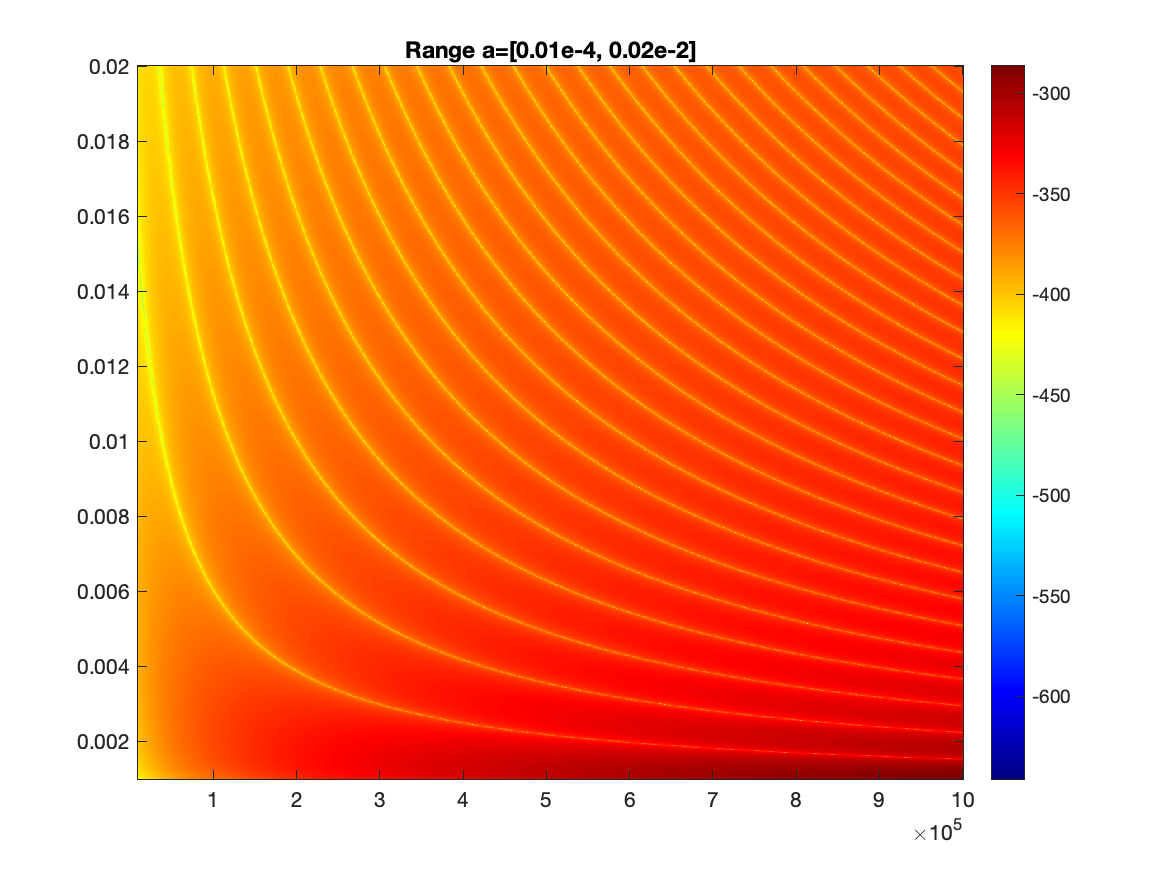
\includegraphics[width=0.7\textwidth]{figures/imagesc_Freq-Radius-TS-1.png}
    \caption{Plot of the frequency and radius against target strength value}
    \label{fig:imagesc_Freq-Radius-TS-1}
\end{figure}

\subsection{Checking hypothesis}
- dependencies on the seed
+filtered, +add.noise, +bubble, -damping

- bandwidth (frequency response is not the same for the bubble, play with ka<<1, identify where is a natural frequency occurrence)

- filtered correlated signal with bubble

- filtered correlated signal without bubble

- with noise filtered with bubble

- with noise filtered without bubble

\subsection{Implementing multiple bubbles distribution}

Simple approach is adapted at first. The same velocity is applied to all bubbles

\begin{itemize}
    
    \item Generation of new bubbles at each time step 

    There are multiple ways of generating bubbles. The first one was to create bubbles in some constrained space using a "rand" for pseudo-random coordinate definition

    In case we want to make a geometry for bubble curtains, we can create a line-frame of the rectangle. Define some discrete amount of points which would act like bubble emitters. Depending on their bubble production performance we can regulate the thickness of created walls.

    \item  Bubble speed 
    
    Speed of the bubble moving at vertical z-direction, where time step can be assumed as 0.1 s:
    \[V_z = \frac{1 m}{n}, \quad 1n \approx 0.1 s\]

    Initially bubbles are generated at the $z=0$ plane and this bubble cloud moves to the surface creating a bubble-flare.

    

    \item Bubble oscillating movement
\end{itemize}

\textbf{Questions:}
\begin{itemize}
    \item When emitted sonar bandwidth contains in its range a resonance frequency of the bubble, the cross-correlation allows to see bubbles gatherings more distinctly?
\end{itemize}

%The following calculations were performed … (equation, substituting variables and consts, result in units)
%
%The mathematical development of calculations is presented below in symbolic form …
%
%Diagram of the experiment
%
%The following diagram is used to identify each element of the setup. It includes representations of measuring instruments, and the geometry of the setup. 
%
%List of the equipment used
%The used setup during the experiment was …
\section{Interpretation}

%The uncertainties associated with measurements were ..
%
%Influencing factors, relationships between variables on the results were …
%
%We have also performed the necessary calculations to validate our hypotheses which consisted of finding the values of …
%
%
%Following the lab instructions we have obtained …

\section{Conclusion}

%The hypotheses of … were validated. 
%
%The proposed solution to the posed problem was …
%
%The objective of the work .. was achieved …
%
%Comparing results from our simulation and calculations with the one obtained from literature are …
%
%The difference between them can be explained with … (due to a manipulation error, protocol design, or the experimental principle) 


\printbibliography
\section*{Appendix: Figures}
\begin{figure} [H] 
    \centering
    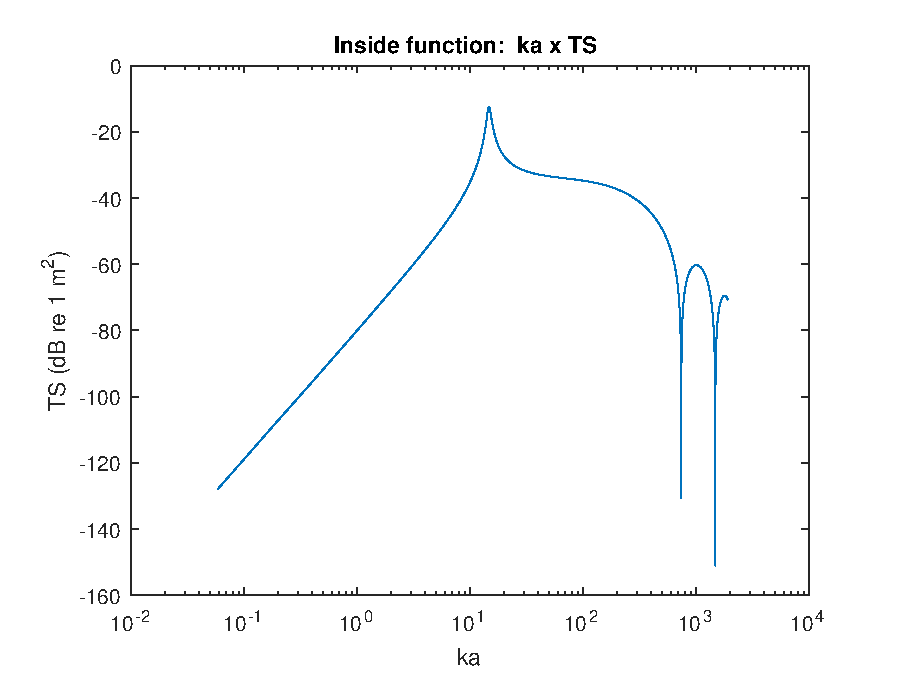
\includegraphics[width=0.7\textwidth]{figures/single-bubble_backscattering-TS.eps}
    \caption{single-bubble_backscattering-TS}
    \label{fig:single-bubble_backscattering-TS}
\end{figure}

\begin{figure} [H]
    \centering
    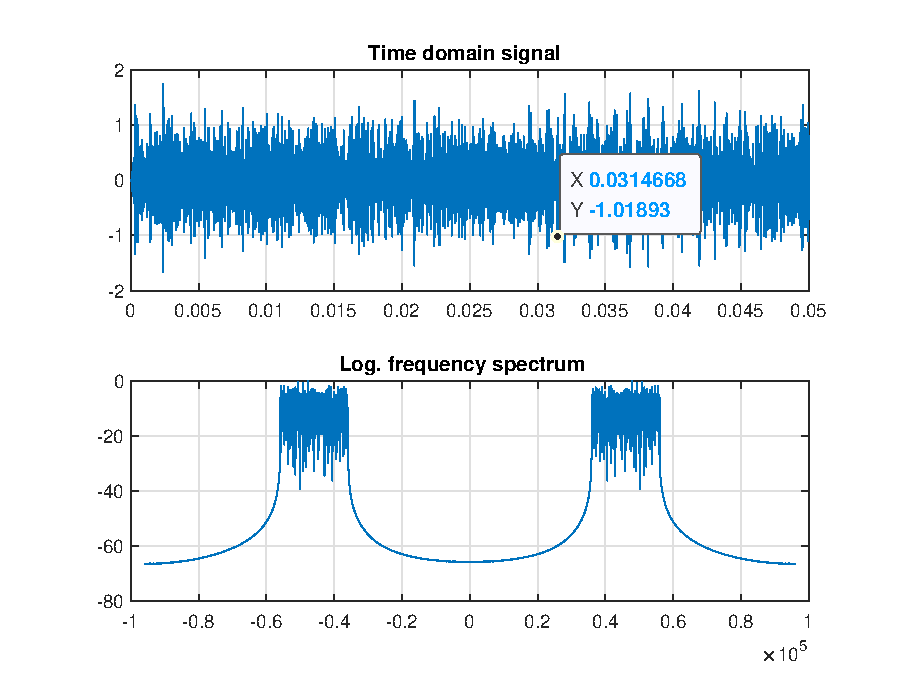
\includegraphics[width=0.7\textwidth]{figures/single-bubble_filtered-time-freq-signal.eps}
    \caption{single-bubble_filtered-time-freq-signal}
    \label{fig:single-bubble_filtered-time-freq-signal}
\end{figure}

\begin{figure} [H]
    \centering
    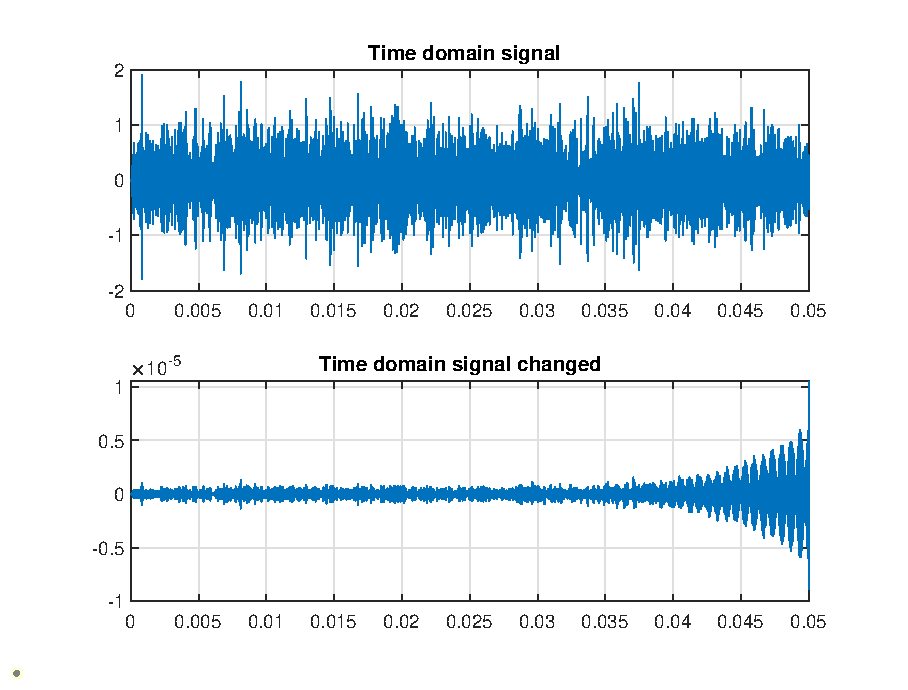
\includegraphics[width=0.7\textwidth]{figures/single-bubble_time_signal_comp.eps}
    \caption{Plot of the single bubble signal in time domain, comparison}
    \label{fig:single-bubble_time_signal_comp.}
\end{figure}

\begin{figure} [H]
    \centering
    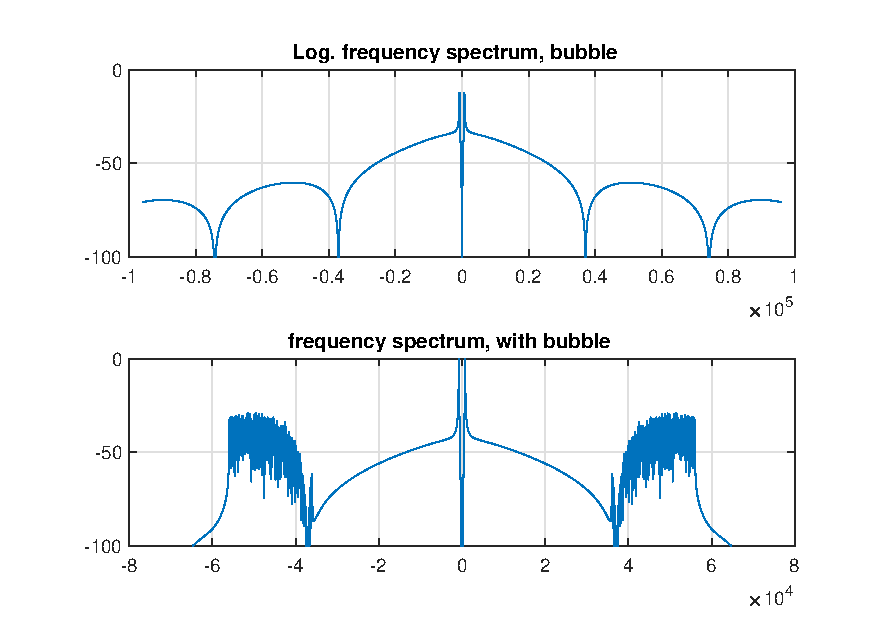
\includegraphics[width=0.7\textwidth]{figures/single-bubble_freq_signal_comp.eps}
    \caption{Plot of the single bubble frequency response, comparison between frequency responses}
    \label{fig:single-bubble_freq_signal_comp}
\end{figure}

\begin{figure} [H]
    \centering
    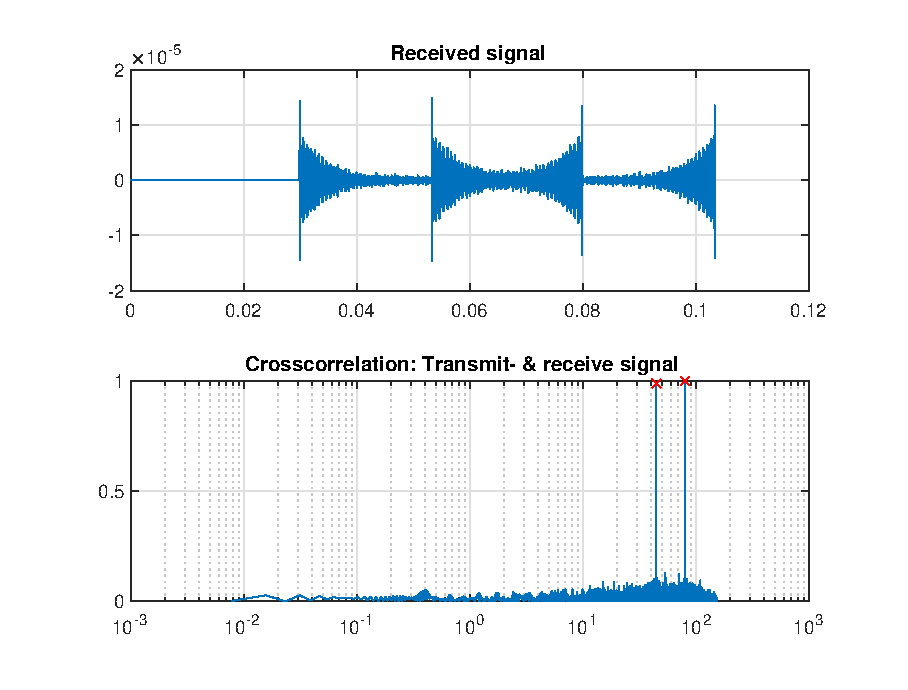
\includegraphics[width=0.7\textwidth]{figures/single-bubble_received-sign_crosscorr.eps}
    \caption{Plot of the single bubble crosscorrelation results}
    \label{fig:single-bubble_received-sign_crosscorr}
\end{figure}

\begin{figure} [H]
    \centering
    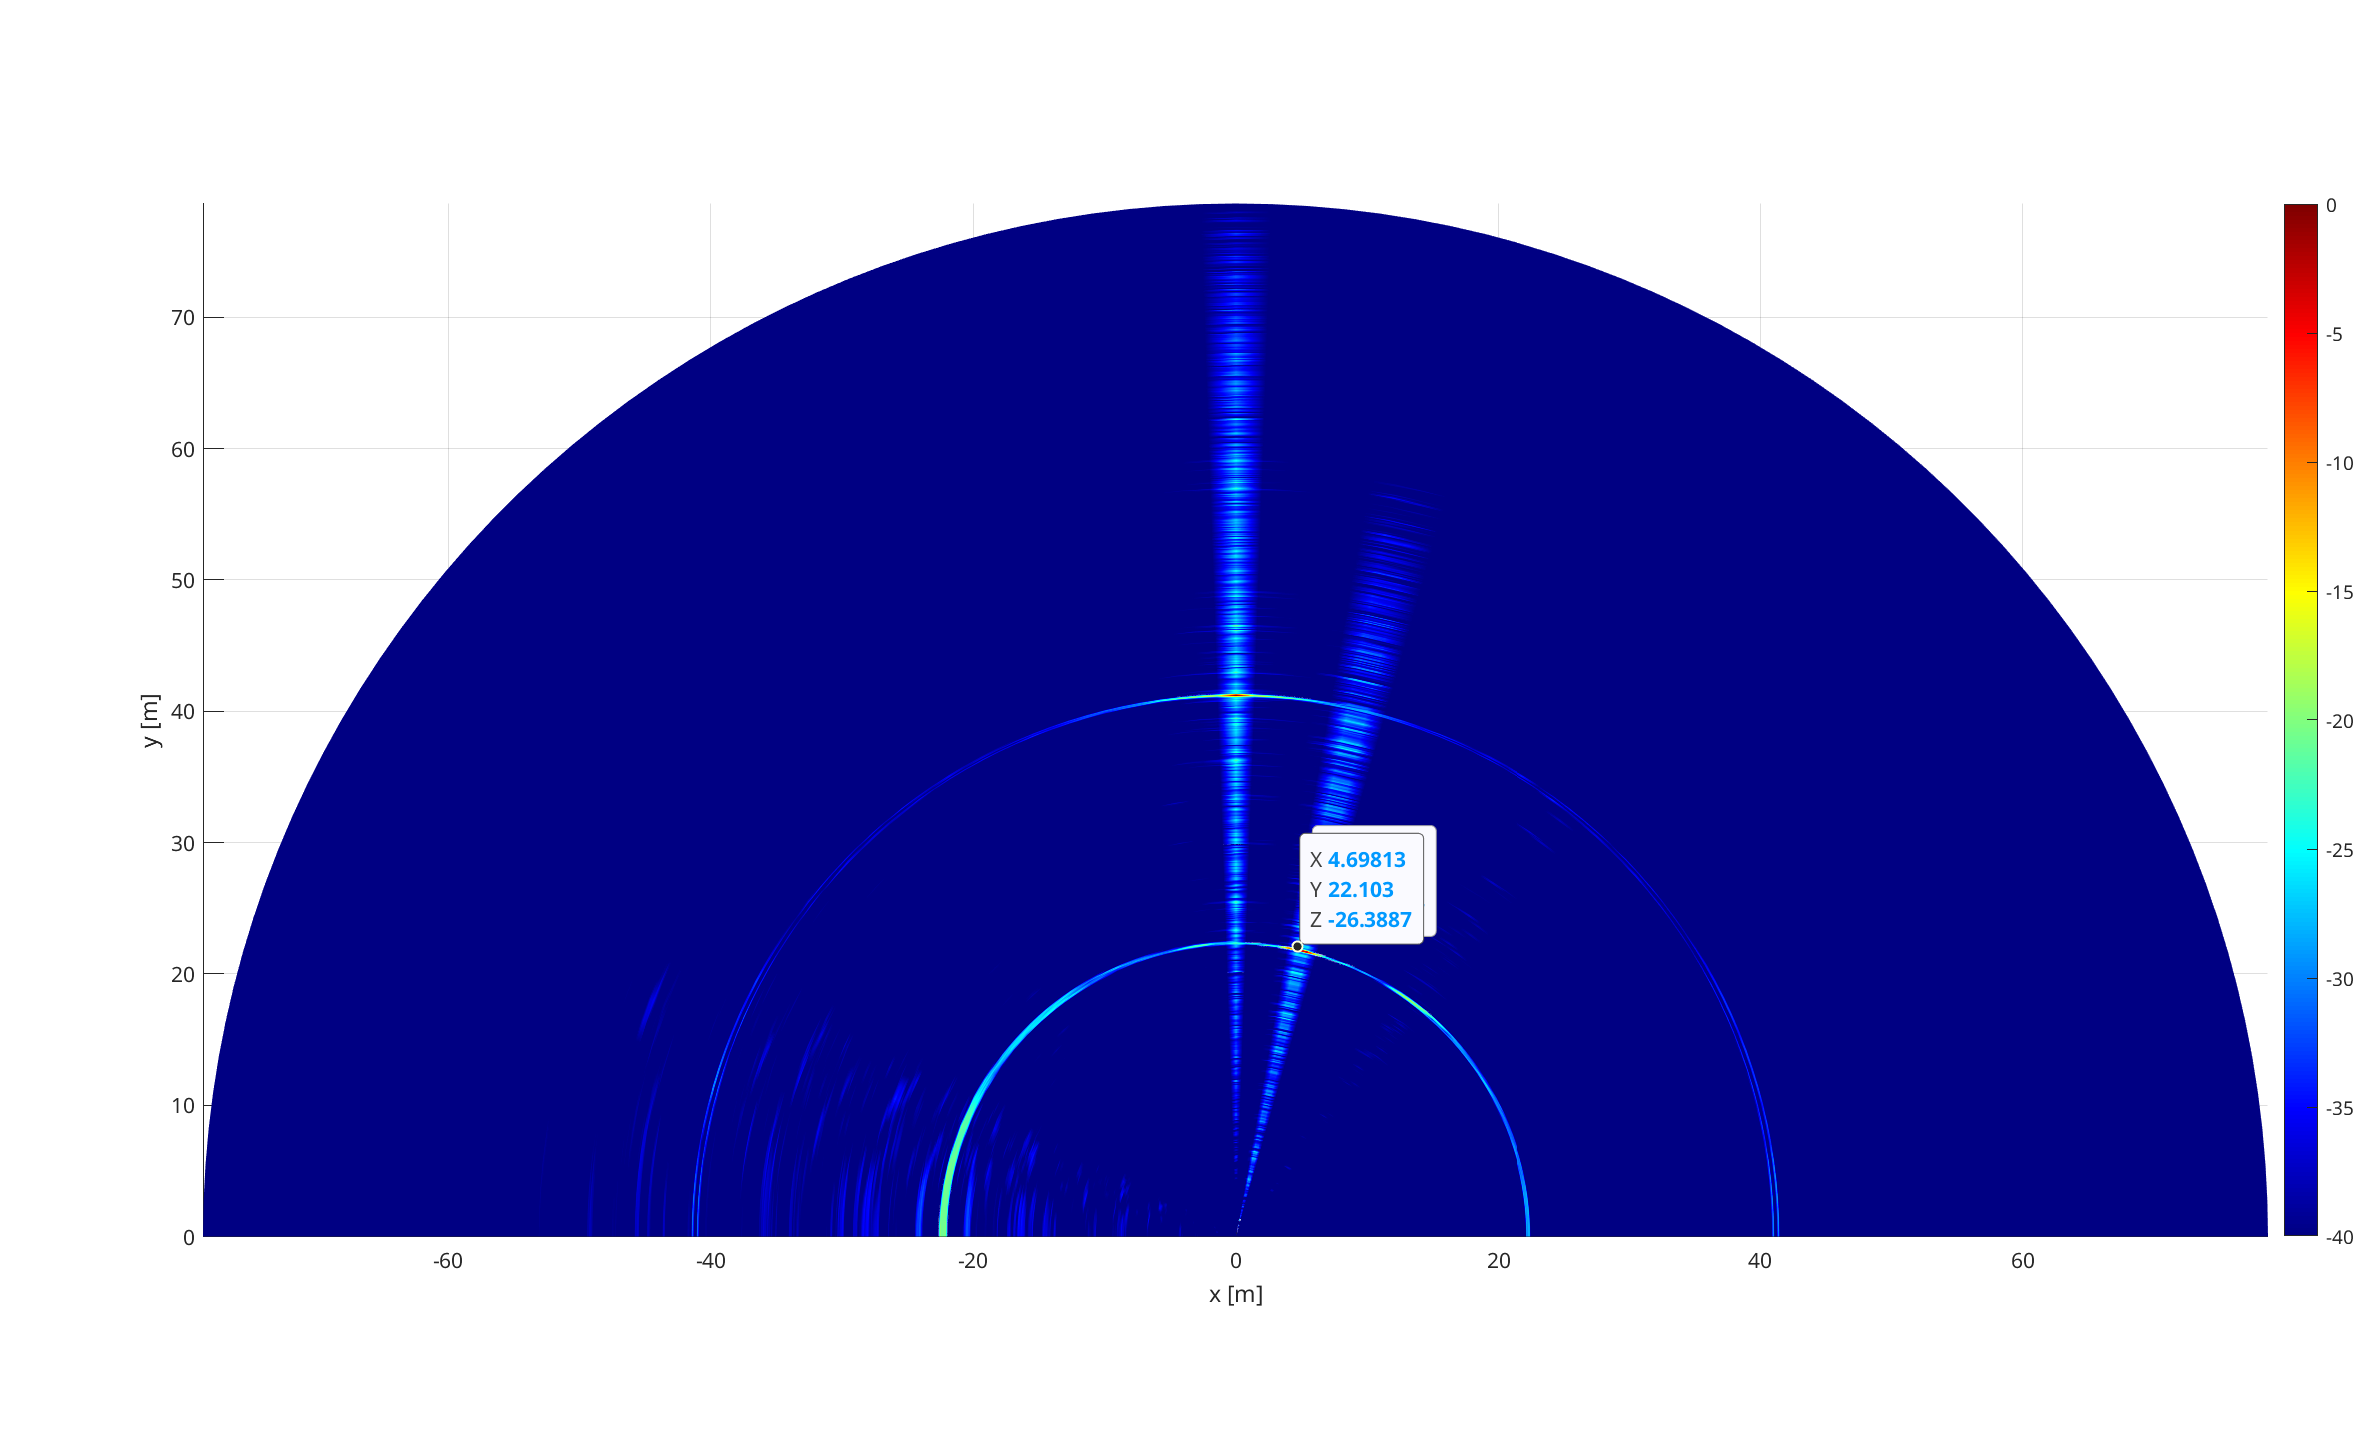
\includegraphics[width=0.7\textwidth]{figures/single-bubble_sonar-resp.eps}
    \caption{Plot of the single bubble sonar response}
    \label{fig:single-bubble_sonar-resp}
\end{figure}

\begin{figure} [H]
    \centering
    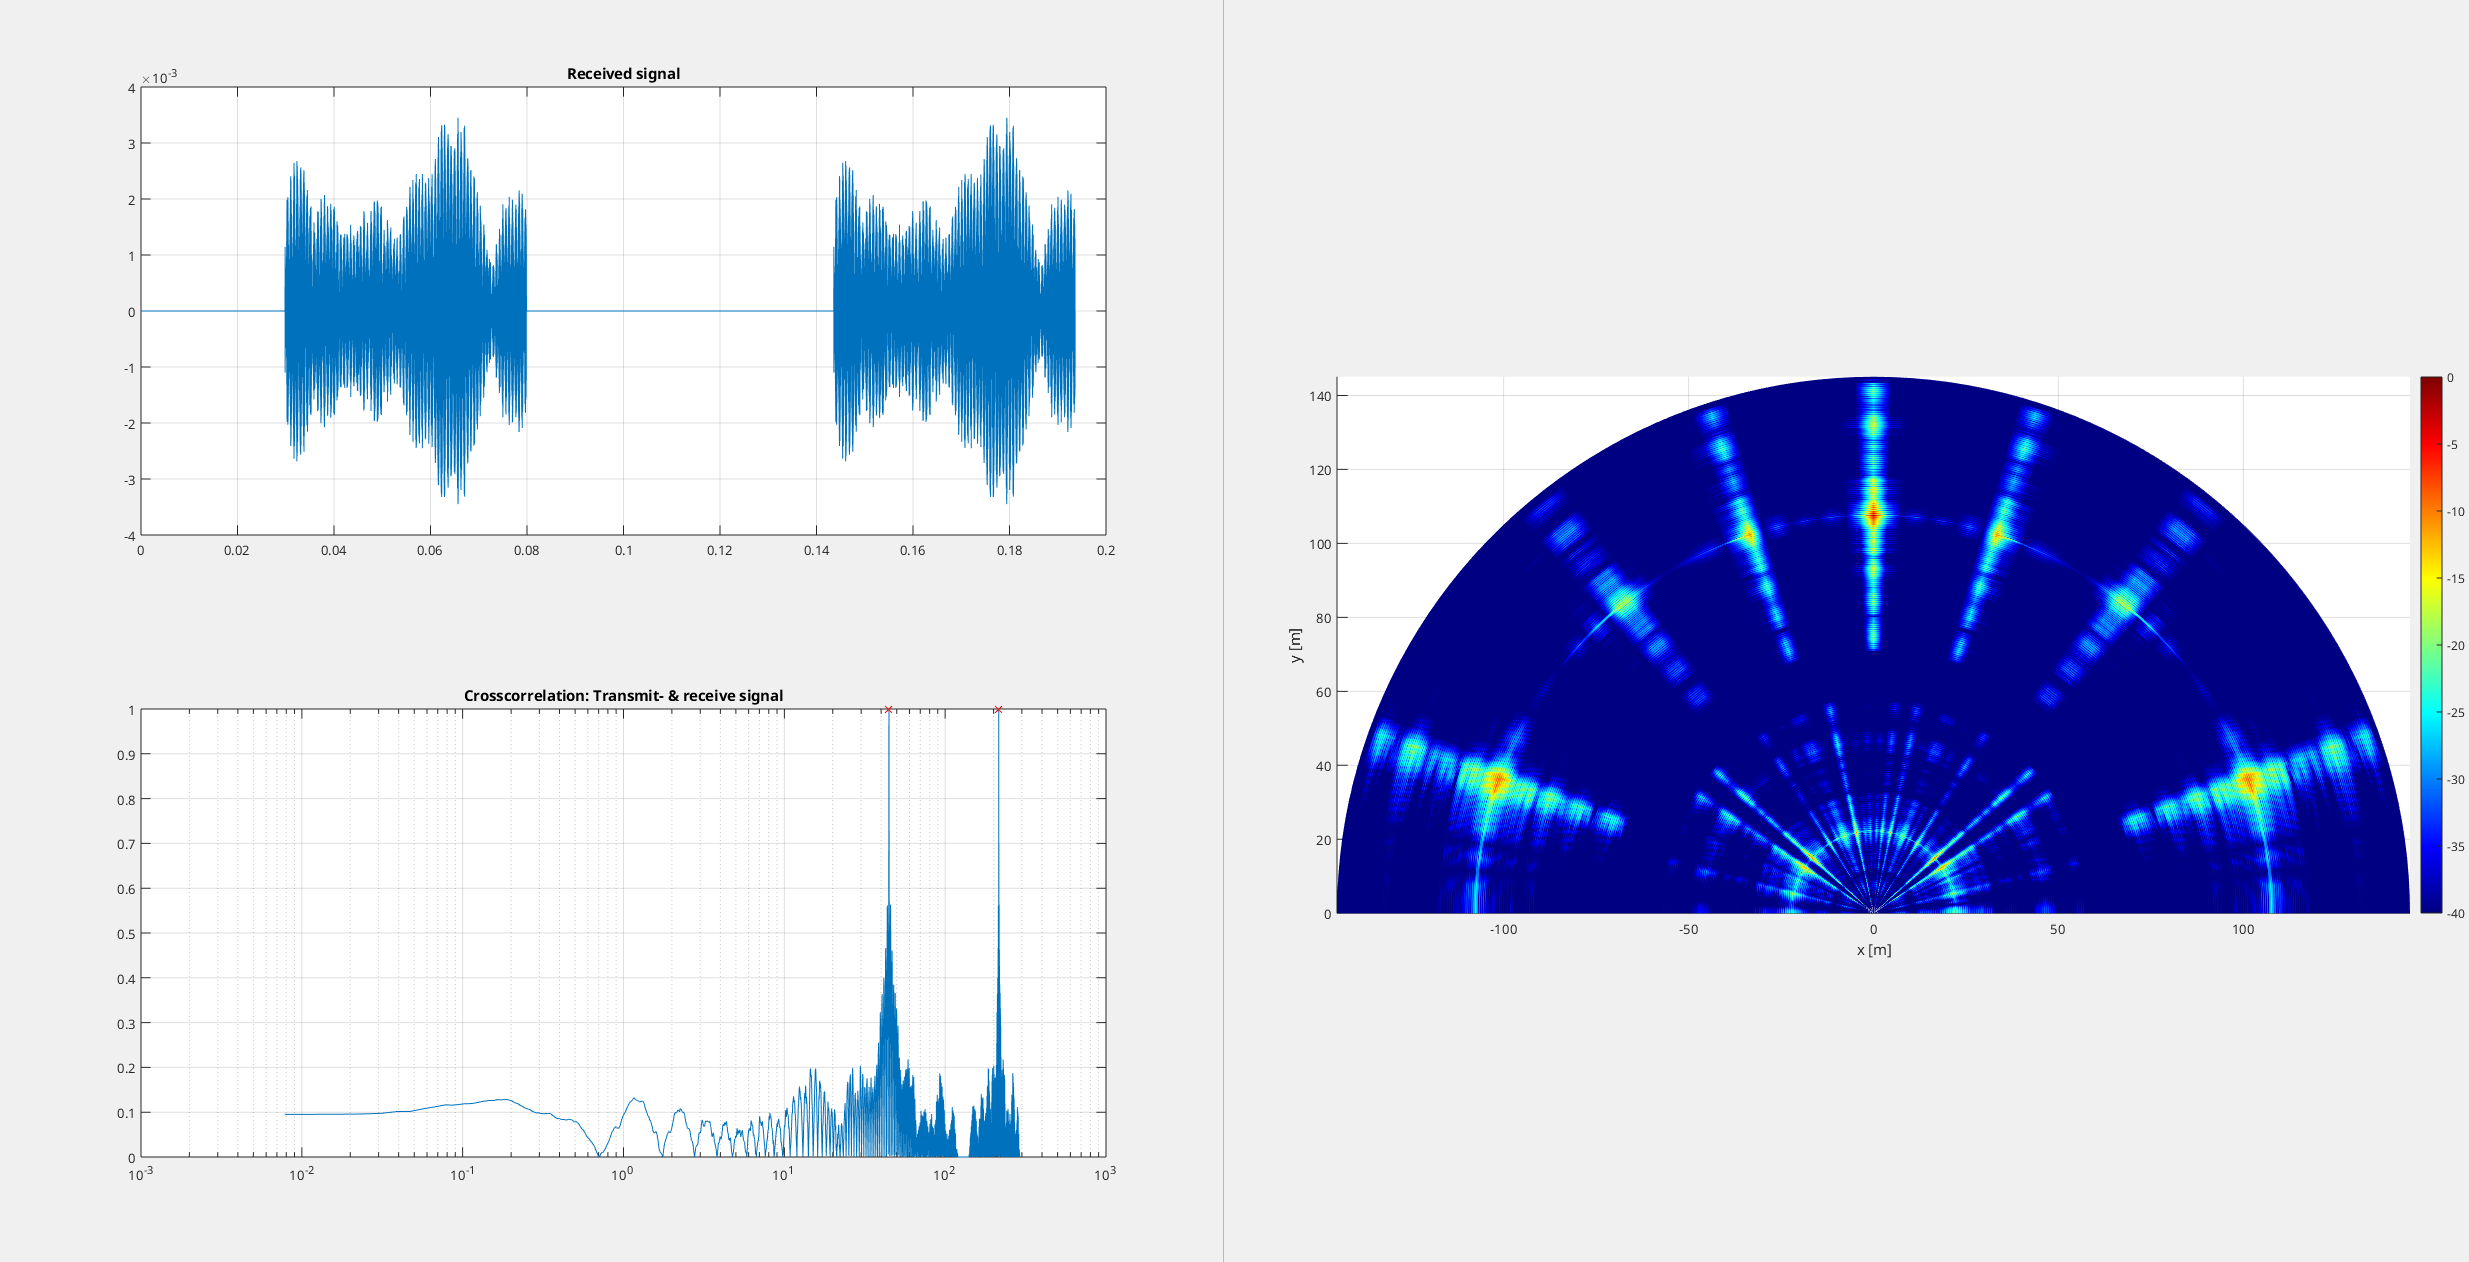
\includegraphics[width=0.7\textwidth]{figures/sonar-nofilter-bubble.png}
    \caption{Plot of the single bubble sonar without filter, but with a bubble response}
    \label{fig:single-bubble_sonar-nofilter-bubble}
\end{figure}

\begin{figure} [H]
    \centering
    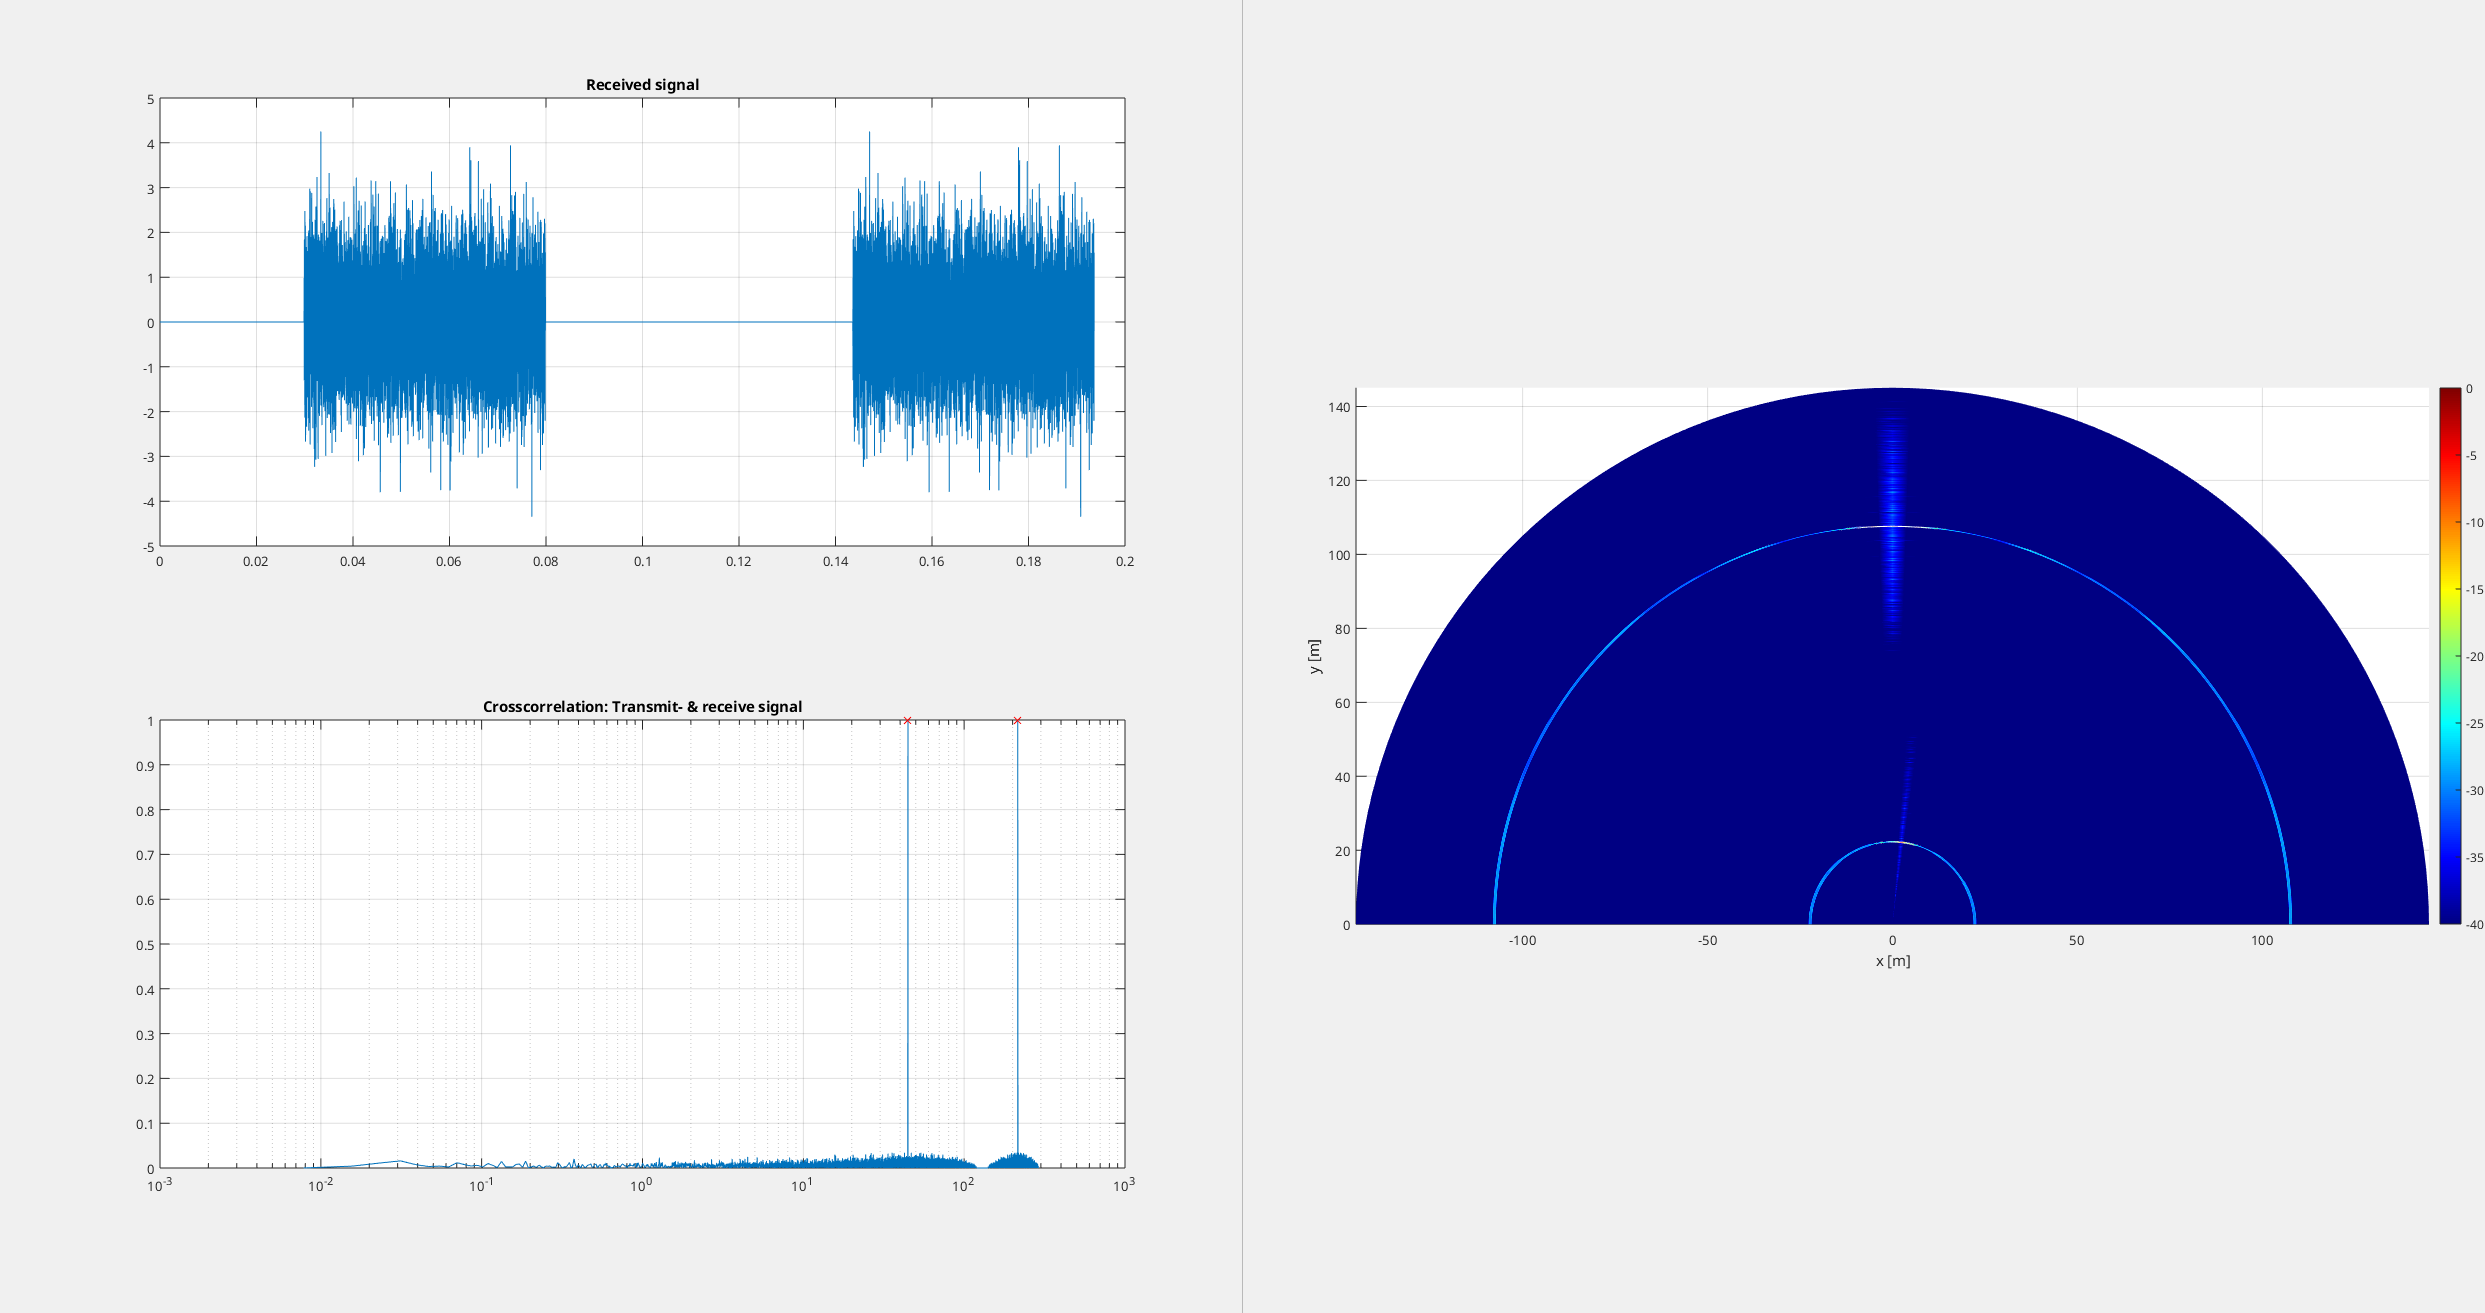
\includegraphics[width=0.7\textwidth]{figures/sonar-nofilter-nobubble.png}
    \caption{Plot of the single bubble sonar without filter and without a bubble response}
    \label{fig:single-bubble_sonar-nofilter-nobubble}
\end{figure}

\begin{figure} [H]
    \centering
    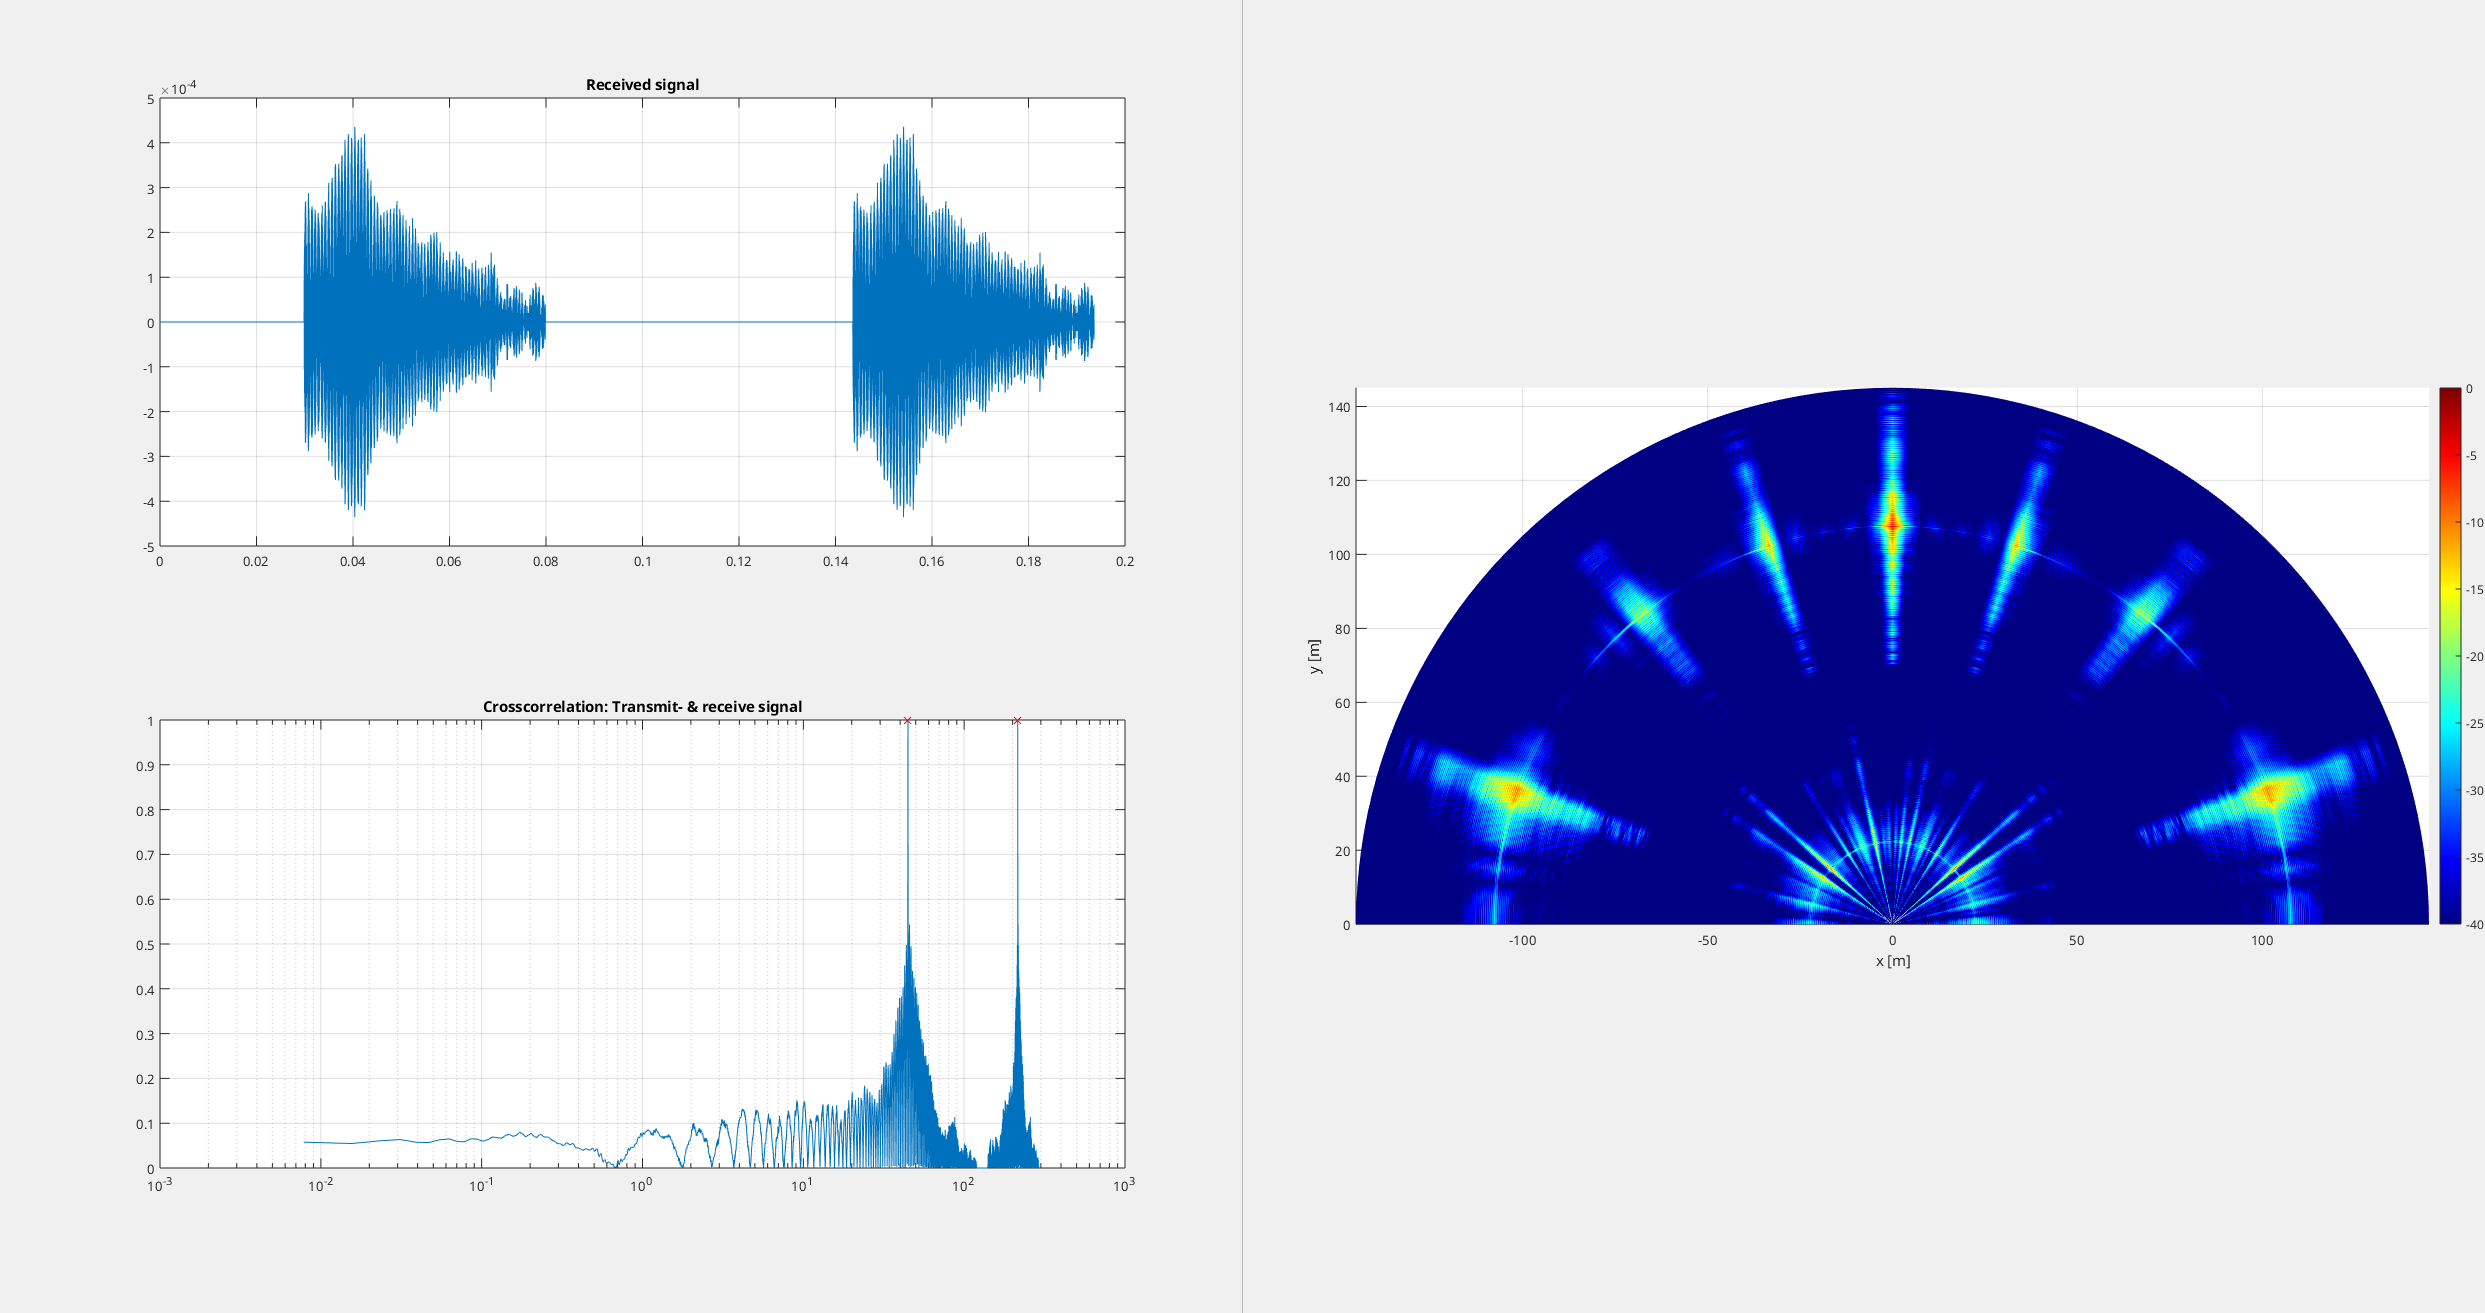
\includegraphics[width=0.7\textwidth]{figures/sonar-addnoise-bubble.png}
    \caption{Plot of the single bubble sonar with filter and additional noise, with a bubble response}
    \label{fig:single-bubble_sonar-addnoise-bubble}
\end{figure}

\begin{figure} [H]
    \centering
    \includegraphics[width=0.7\textwidth]{'figures2/Sonar_Animation1.gif'}
    \caption{Sonar animation of multiple bubbles}
    \label{fig:Sonar_Animation1}
\end{figure}
\begin{figure} [H]
    \centering
    \includegraphics[width=0.7\textwidth]{figures2/Bubble_mov3.gif}
    \caption{Animation of multiple bubbles flare creation}
    \label{fig:Bubble_mov3}
\end{figure}

%graphs, tables, or any other type of figures that address the issue. 
%
%Figures should be accompanied by a title and an explanatory legend, similar to tables. 
%
%Don't forget to specify the nature and units. 
%Use a scale that maximizes the use of the surface area.


\end{document}
